%%%%%%%%%%%%%%%
% This is the main file for compiling the LaTeX document.
%
% Please keep all sections in there respective files and compile
% the document from here.
%%%%%%%%%%%%%%%

\documentclass[pdftex,12pt]{article}

\usepackage{fancyhdr}	% For header and footers.
\usepackage{graphicx}	% For including images.
\usepackage[colorlinks,bookmarksnumbered,linktocpage]{hyperref}	% For links to sections in TOC.

\renewcommand{\footrulewidth}{0.4pt}
%\renewcommand{\footrulewidth}{0.4pt}
\pagestyle{fancy}	% To use the fancyhdr package.


% Finally the actual document we're concerned with.
\begin{document}

	%%%%%%%%%%%%%%%
% This file is concerned with the title page.
%
% Please remember to compile the document from "00_finalreport.tex".
% It will not work otherwise.
%%%%%%%%%%%%%%%

\begin{titlepage}
	\begin{center}

		% Upper part of the page with our beautiful logo.
		
\includegraphics[width=0.40\textwidth]{./logo.png}\\[1cm]

		% text below image.
		\textsc{\large Web UI Team}\\[1.5cm]

		% two horizontal lines with some text between.
		\HRule \\[0.4cm]
			{\huge \bfseries Final Report}\\[0.4cm]
		\HRule \\[1.5cm]

		\emph{Members:}\\
		Aryn \textsc{Grause}\\
		Garrett \textsc{Dieckmann}\\
		Katie \textsc{Mueller}\\
		Kyle \textsc{Monnett}\\
		
		% Blank space to the bottom of page.
		\vfill

		% Bottom of the page.
		{\large \today}
		
	\end{center}
\end{titlepage}			% Done!
	
	% Just here to enter a completely blank page.
	\thispagestyle{empty}
		\mbox{}
	\newpage

	\tableofcontents				% Auto-done!
	\newpage
	
	% Just here to enter a completely blank page.
	\thispagestyle{empty}
		\mbox{}
	\newpage

	%%%%%%%%%%%%%%%
% This file is concerned with the end product description.
%
% Please remember to compile the document from "00_finalreport.tex".
% It will not work otherwise.
%%%%%%%%%%%%%%%

\section{End Product Description}
	As the Web User Interface team for VirPong, our end product is a direct portal through which users of VirPong can watch VirPong games (both live and past matches) and access game information including high scores and current rankings for VirPong players. The website will also serve as a front end to VirPong, allowing new users to explore the VirPong world and become active in it. Therefore, our goal with the VirPong website is to provide an attractive and intuitive portal into the world of VirPong.\\In producing the VirPong website, we will be working on various aspects that are essential to the success of the VirPong experience. A portion of the website will be dedicated to viewing VirPong games, whether these games have already been played by VirPong users or are happening in real time, by using the VirPong mobile applications. Another part of the website will be dedicated to the user experience, providing a space for users to update their personal information. No sports experience would be complete without access to top scores, as well as following our favorite player, so there will also be a section of the VirPong website that will showcase high scoring games, as well as statistics about certain VirPong �power players.�\\In constructing the VirPong platform, we also want to create an Open Source project that will break into the competitive sports industry, thus we want to focus on creating a solution that will be adaptable for other developers. To achieve this goal, our team will work on VirPong knowing that other developers will be using our code, and will provide in-line comments as well as documentation to make VirPong easy to redeploy. Specifically, we are maintaining install guides that document every technology, as well as the install instructions for these technologies, so that other developers can quickly redeploy VirPong by following a set of instructions tailored explicitly for the VirPong platform. To make the VirPong project easy to download, all of the source code has been pushed to GitHub and the VirPong team will continue to update VirPong code to include more features, as well as update VirPong to conform to current standards of the web.

\newpage		% Incomplete

	%%%%%%%%%%%%%%%
% This file is concerned with the functional requirements.
% Since this section is a little larger than the others,
% it has been broken down into two other files for ease of editing.
%
% Please remember to compile the document from "00_finalreport.tex".
% It will not work otherwise.
%%%%%%%%%%%%%%%

\section{Functional Requirements}
	
	%%%%%%%%%%%%%%%
% This file is concerned with the use cases,
% a subsection of the functional requirements.
%
% Please remember to compile the document from "00_finalreport.tex".
% It will not work otherwise.
%%%%%%%%%%%%%%%

	\subsection{Use Cases}
	
		\phantomsection
		\addcontentsline{toc}{subsubsection}{Registering for an Account}
		\subsubsection*{Registering for an Account}
		Title: Successful Registration for the Game\\
		Actors: User, Data Repository, System\\
		Preconditions:
		\begin{itemize}
			\item Computer System (in its �on� state).
			\item User has the ability to navigate on the computer.
			%\item User understands English and is literate.
		\end{itemize}
		
		Post Conditions:
		\begin{itemize}
			\item User is successfully registered for the site.
		\end{itemize}
		
		Main Success Scenario:
		\begin{description}
			%\item[1.] User navigates to the System.
			\item[1.] User fills out appropriate information on System�s form.
			\item[2.] System connects to Data Repository.
			\item[3.] System checks for duplicate information.
			\item[4.] Requests differnt information if duplicate found.
			\item[5.] System stores information in Data Repository.
			\item[6.] System disconnects from Data Repository.
			\item[7.] System reports successful registration.
		\end{description}
		
		Extensions:
		\begin{description}
			\item[1.] User navigates to the System.
			\begin{description}
			
				\item[1a.] System is down.
				\begin{description}
					\item[1.] Be sad.
					\item[2.] Fix system.
				\end{description}
			\end{description}
			
			\item[2.] User fills out appropriate information on System�s form
			\begin{description}
				\item[2a.] Users fills out information incorrectly (e.g. enters street name instead of birthday)
				\begin{description}
					\item[1.] Validate form before accepting
					\item[2.] Report failed validation (e.g. incorrect information for the following field)
				\end{description}
				\item[2b.] Username information already exists
				\begin{description}
					\item[1.] Check Data Repository for identical usernames
					\item[2.] Inform User that the username is already taken
					\item[3.] Prompts User to register with a unique username
				\end{description}
			\end{description}
			
			\item[3.] System connects to Data Repository
			\begin{description}
				\item[3a.] Failed connection
				\begin{description}
					\item[1.] Ask user to refresh system
				\end{description}
				\item[3b.] Second failed connection
				\begin{description}
					\item[1.] Ask user to contact VirPong and report an error
					\item[2.] Provide user with a link to the Contact Us page
				\end{description}
			\end{description}
			
			\item[4.] System stores information in Data Repository
			\begin{description}
				\item[4a.] Information is not stored in repository due to repository going down
				\begin{description}
					\item[1.] Report an error stating that this service is not available and to return at another time
				\end{description}
				\item[4b.] Repository throws an error
				\begin{description}
					\item[1.] Ask user to try again
				\end{description}
				\item[4c.] Repository throws an error a second time
				\begin{description}
					\item[1.] Ask user to contact VirPong and report an error
					\item[2.] Provide user with a link to the Contact Us page
				\end{description}
			\end{description}
			
			\item[5.] System disconnects from Data Repository
			\begin{description}
				\item[5a.] Disconnection failed
				\begin{description}
					\item[1.] Terminate through the use of exception handling
				\end{description}
			\end{description}
		\end{description}
		
		
		\phantomsection
		\addcontentsline{toc}{subsubsection}{Watch Live}
		\subsubsection*{Watch Live}Title: Successful Live Game Viewing\\Actors: User, Game Manager, System\\
		Preconditions:
		\begin{itemize}
			\item Computer System (in its �on� state)
			\item User has the ability to navigate on the computer
			%\item User understands English and is literate
		\end{itemize}
		
		Post Conditions:
		\begin{itemize}
			\item User sucessfully watches game without errors
		\end{itemize}
		
		Main Success Scenario:
		\begin{description}
			\item[1.] User navigates to the System
			\item[2.] System display options to user.
			\item[3.] User selects the game information to view
			\item[4.] System connects to the Game Manager
			\item[5.] System informs Game Manager of which game was selected by user
			\item[6.] Game Manager supplies information on the selected game to the system
			\item[7.] System displays information
			\item[8.] Repeat 4, 5, 6, and 7 until information stream ends from Game Manager
			\item[9.] System closes connection to the Game Manager
			\item[10.] System informs User that the game is over
		\end{description}
		
		Extensions:
		\begin{description}
			\item[1.] User navigates to the System
			\begin{description}
				\item[1a.] System is down
				\begin{description}
					\item[1.] Report 404 Error that provides information to the User
				\end{description}
			\end{description}
			
			\item[2.] User selects the game information to view
			\begin{description}
				\item[2a.] User isn't doing much
				\begin{description}
					\item[1.] Suggest a current game to view
				\end{description}
				\item[2b.] No games are available
				\begin{description}
					\item[1.] Print an apologetic message stating that no current games are available
					\item[2.] Suggest some historical games to view
				\end{description}
			\end{description}
			
			\item[3.] System connects to the Game Manager
			\begin{description}
				\item[3a.] Unsuccessful connection
				\begin{description}
					\item[1.] Ask user to refresh system
				\end{description}
				\item[3b.] Second unsuccessful connections
				\begin{description}
					\item[1.] Ask user to contact VirPong and report an error
					\item[2.] Provide user with a link to the Contact Us page
				\end{description}
			\end{description}
			
			\item[4.] System informs Game Manager of which game was selected by user
			\begin{description}
				\item[4a.] System does not inform the Game Manager within allotted time
				\begin{description}
					\item[1.] Restart connection with the Game Manager
				\end{description}
				\item[4b.] System fails to inform the Game Manager a second time
				\begin{description}
					\item[1.] Ask user to refresh system
				\end{description}
				\item[4c.] System continues to fail
				\begin{description}
					\item[1.] Ask user to contact VirPong and report an error
					\item[2.] Provide user with a link to the Contact Us page
				\end{description}
			\end{description}
			
			\item[5.] Game Manager supplies information on the selected game to the system
			\begin{description}
				\item[5a.] Information on the wrong game is provided
				\begin{description}
					\item[1.] Provide the user with the ability to leave a game at any moment
				\end{description}
				\item[5b.] No information is supplied
				\begin{description}
					\item[1.] Ask user to refresh system
				\end{description}
				\item[5c.] No information was provided a second time
				\begin{description}
					\item[1.] Ask user to contact VirPong and report an error
					\item[2.] Provide user with a link to the Contact Us page
				\end{description}
			\end{description}
			
%			\item[6.] System interprets the information
%			\begin{description}
%				\item[6a.] Information is in a different format
%				\begin{description}
%					\item[1.] Ask user to refresh system
%				\end{description}
%				\item[6b.] Information is in a different format a second time
%				\begin{description}
%					\item[1.] Ask user to contact VirPong and report an error
%					\item[2.] Provide user with a link to the Contact Us page
%				\end{description}
%			\end{description}
			
			\item[7.] System displays information
			\begin{description}
				\item[7a.] System is not supported by the user�s browser
				\begin{description}
					\item[1.] Check which browser the user is using
					\item[2.] Provide suggestion for a compatible browser
				\end{description}
			\end{description}
			
			\item[8.] Repeat 4, 5, 6, and 7 until information stream ends from Game Manager
			\begin{description}
				\item[8a.] No new event has occurred in an allotted time period
				\begin{description}
					\item[1.] Close connection with the Game Manager
				\end{description}
			\end{description}
			
			\item[9.] System closes connection to the Game Manager
			\begin{description}
				\item[9a.] Connection is not closed in an allotted time
				\begin{description}
					\item[1.] Reattempt to close connection
				\end{description}
			\end{description}
			
			\item[10.] System informs User that the game is over
			\begin{description}
				\item[10a.] System does not inform user
				\begin{description}
					\item[1.] Provide navigation to other services
				\end{description}
			\end{description}
		\end{description}
		
		
		\phantomsection
		\addcontentsline{toc}{subsubsection}{Signing-In}
		\subsubsection*{Signing-In}Title: Successful Sign-In Attempt\\Actors: User, Data Repository, System\\
		Preconditions:
		\begin{itemize}
			\item Computer System (in its �on� state)
			\item Ability to Navigate to the system
			%\item User understands English
		\end{itemize}
		Post Conditions:
		\begin{itemize}
			\item User is signed in to the system
		\end{itemize}
		
		Main Success Scenario:
		\begin{enumerate}
			\item User navigates to the System
			\item User fills out appropriate information on System�s sign-in
			\item System connects to Data Repository
			\item System confirms user input with information in Data Repository
			\item System disconnects from Data Repository
			\item System reports successful sign-in
		\end{enumerate}
		
		Extensions:
		\begin{description}
			\item[1.] User navigates to the System
			\begin{description}
				\item[1a.] System is down
				\begin{description}
					\item[1.] Report 404 Error that provides information to the User
				\end{description}
			\end{description}
			
			\item[3.] System connects to Data Repository
			\begin{description}
				\item[3a.] Failed connection
				\begin{description}
					\item[1.] Ask user to refresh system
				\end{description}
				\item[3b.] Failed connection a second time
				\begin{description}
					\item[1.] Ask user to contact VirPong and report an error
					\item[2.] Provide user with a link to the Contact Us page
				\end{description}
			\end{description}
			
			\item[4.] System confirms user input with information in Data Repository
			\begin{description}
				\item[4a.] User input is incorrect and does not match repository
				\begin{description}
					\item[1.] Report an error message stating unable to log-in
					\item[2.] Prompt the user to try authenticating again
				\end{description}
				\item[4b.] User does not exist
				\begin{description}
					\item[1.] Report an error message stating unable to log-in
					\item[2.] Prompt the user to try authenticating again
				\end{description}
				\item[4c.] Repository throws an error
				\begin{description}
					\item[1.] Ask user to refresh system
				\end{description}
				\item[4d.] Repository throws an error a second time
				\begin{description}
					\item[1.] Ask user to contact VirPong and report an error
					\item[2.] Provide user with a link to the Contact Us page
				\end{description}
			\end{description}
			
			\item[5.] System disconnects from Data Repository
			\begin{description}
				\item[5a.] Disconnection failed
				\begin{description}
					\item[1.] Terminate through the use of exception handling
				\end{description}
			\end{description}
		\end{description}
		
		
		\phantomsection
		\addcontentsline{toc}{subsubsection}{Change Account Settings}
		\subsubsection*{Change Account Settings}Title: Successful Modification of Account Settings\\Actors: User, Data Repository, System
		Preconditions:
		\begin{itemize}
			\item Computer System (in its �on� state)
			\item User has the ability to navigate on the computer
			%\item User understands English and is literate
		\end{itemize}
		Post Conditions:
		\begin{itemize}
			\item User successfully changes settings of their account
		\end{itemize}
		
		Main Success Scenario:
		\begin{enumerate}
			\item User navigates to the System
			\item User authenticates into the System
			\item User changes information
			\item System connects to Data Repository
			\item System provides updated feedback to Data Repository
			\item System Disconnects from Data Repository
			\item System relays successful changes
		\end{enumerate}

		Extensions:
		\begin{description}
			\item[1.] User authenticates into the System
			\begin{description}
				\item[1a.] User is not registered to use system
				\begin{description}
					\item[1.] Report an error message stating unable to log-in
					\item[2.] Prompt the user to try authenticating again
				\end{description}
			\end{description}
			\begin{description}
				\item[1b.] Authentication fail
				\begin{description}
					\item[1.] Report an error message stating unable to log-in
					\item[2.] Prompt the user to try authenticating again
				\end{description}
			\end{description}
		\end{description}
		\begin{description}
			\item[2.] User navigates to the System
			\begin{description}
				\item[2a.] System is down
				\begin{description}
					\item[1.] Report 404 Error that provides information to the User
				\end{description}
			\end{description}
		\end{description}
		\begin{description}
			\item[3.] User changes information
			\begin{description}
				\item[3a.] User provides wrong type of information (ex. a name instead of a date for the birthday field
				\begin{description}
					\item[1.] Validate form upon submission
					\item[2.] Report failed validation issues (aka. incorrect information for the following field)
				\end{description}
			\end{description}
		\end{description}
		\begin{description}
			\item[4.] System connects to Data Repository
				\begin{description}
					\item[4a.] Repository throws an error
					\begin{description}
						\item[1.] Ask user to refresh system
					\end{description}
					\item[4b.] Repository throws an error a second time
					\begin{description}
						\item[1.] Ask user to contact VirPong and report an error
						\item[2.] Provide user with a link to the Contact Us page
					\end{description}
				\end{description}
		\end{description}
		\begin{description}
			\item[5.] System provides updated feedback to Data Repository
				\begin{description}
					\item[5a.] Information does not get passed to the Data Repository
					\begin{description}
						\item[1.] Notify user that the information was not updated
						\item[2.] Navigates user to Step 3
					\end{description}
					\item[5b.] Connection breaks
					\begin{description}
						\item[1.] Ask user to refresh system
					\end{description}
					\item[5c.] Connection breaks a second time
					\begin{description}
						\item[1.] Ask user to contact VirPong and report an error
						\item[2.] Provide user with a link to the Contact Us page
					\end{description}
				\end{description}
		\end{description}
		\begin{description}
			\item[6.] System Disconnects from Data Repository
			\begin{description}
				\item[6a.] Disconnection failed
				\begin{description}
					\item[1.] Terminate through the use of exception handling
				\end{description}
			\end{description}
		\end{description}


		\phantomsection
		\addcontentsline{toc}{subsubsection}{Look Up Player History}
		\subsubsection*{Look Up Player History}Title: Successful Viewing of Player History\\Actors: User, Data Repository, System\\
		Preconditions:
		\begin{itemize}
			\item Computer System (in its �on� state)
			\item User has the ability to navigate on the computer
			%\item User understands English and is literate
		\end{itemize}

		Post Conditions:
		\begin{itemize}
			\item User successfully views their player history
		\end{itemize}

		Main Success Scenario:
		\begin{enumerate}
			\item User navigates to the System
			\item User authenticates into the System
			\item System connects to Data Repository
			\item System asks for information from Data Repository
			\item Data Repository sends requested information to System
			\item System Disconnects from Data Repository
			\item System displays information
			\item User reads their game information
		\end{enumerate}

		Extensions:
		\begin{description}
			\item[1.] User authenticates into the System
			\begin{description}
				\item[1a.] User is not registered to use system
				\begin{description}
					\item[1.] Report an error message stating unable to log-in
					\item[2.] Prompt the user to try authenticating again
				\end{description}
				\item[1b.] Authentication fail
				\begin{description}
					\item[1.] Report an error message stating unable to log-in
					\item[2.] Prompt the user to try authenticating again
				\end{description}
			\end{description}
			\item[2.] User navigates to the System
			\begin{description}
				\item[2a.] System is down
				\begin{description}
					\item[1.] Report 404 Error that provides information to the User
				\end{description}
			\end{description}
			\item[3.] System connects to Data Repository
			\begin{description}
				\item[3a.] Repository throws an error
				\begin{description}
					\item[1.] Ask user to refresh system
				\end{description}
				\item[3b.] Repository throws an error a second time
				\begin{description}
					\item[1.] Ask user to contact VirPong and report an error
					\item[2.] Provide user with a link to the Contact Us page
				\end{description}
			\end{description}
			\item[4.] System asks for information from Data Repository
			\begin{description}
				\item[4a.] Request for information does not get made
				\begin{description}
					\item[1.] Report an error stating that this service is not available and to return at another time
				\end{description}
				\item[4b.] Connection breaks
				\begin{description}
					\item[1.] Report an error stating that this service is not available and to return at another time
				\end{description}
				\item[4c.] Repository throws an error
				\begin{description}
					\item[1.] Ask user to refresh system
				\end{description}
				\item[4d.] Repository throws an error a second time
				\begin{description}
					\item[1.] Ask user to contact VirPong and report an error
					\item[2.] Provide user with a link to the Contact Us page
				\end{description}
			\end{description}
			\item[5.] Data Repository sends requested information to System
			\begin{description}
				\item[5a.] Source sends wrong information
				\begin{description}
					\item[1.] Check information for proper format
					\item[2.] Display an error message
					\item[3.] Ask user to refresh system
				\end{description}
				\item[5b.] Source sends wrong information a second time
				\begin{description}
					\item[1.] Ask user to contact VirPong and report an error
					\item[2.] Provide user with a link to the Contact Us page
				\end{description}
				\item[5c.] Source sends no information
				\begin{description}
					\item[1.] Check information for proper format
					\item[2.] Display an error message
					\item[3.] Ask user to refresh system
				\end{description}
				\item[5d.] Source sends no information a second time
				\begin{description}
					\item[1.] Ask user to contact VirPong and report an error
					\item[2.] Provide user with a link to the Contact Us page
				\end{description}
			\end{description}
			\item[6.] System Disconnects from Data Repository
			\begin{description}
				\item[6a.] Disconnection fails
				\begin{description}
					\item[1.] Terminate through the use of exception handling
				\end{description}
			\end{description}
			\item[7.] System displays information
			\begin{description}
				\item[7a.] System cannot interpret the information
				\begin{description}
					\item[1.] Check information for proper format
					\item[2.] Display an error message
					\item[3.] Ask user to refresh system
				\end{description}
			\end{description}
		\end{description}


		\phantomsection
		\addcontentsline{toc}{subsubsection}{Player Plays in a Tournament}
		\subsubsection*{Player Plays in a Tournament}Title: Successful Participation in Tournament\\Actors: Company, User, Data Repository, System\\
		Preconditions: 
		\begin{itemize}
			\item Computer System (in its �on� state)
			\item User has the ability to navigate on the computer
			%\item User understands English and is literate
		\end{itemize}
		
		Post Conditions:
		\begin{itemize}
			\item User successfully plays in tournament
		\end{itemize}

		Main Success Scenario:
		\begin{enumerate}
			\item Company decides to host a tournament
			\item User authenticates into the System
			\item System displays tournament Registration
			\item User navigates to the System
			\item User requests System they would like to register for a tournament
			\item System connects to Data Repository
			\item System registers User on Data Repository 
			\item System Disconnects from Data Repository
			\item System confirms registration
			\item System sends a reminder to User
			%\item User authenticates into System
			\item User navigates to game system
			\item User successfully plays a game
		\end{enumerate}

		Extensions:
		\begin{description}
			\item[3.] User authenticates into the System
			\begin{description}
				\item[3a.] User is not registered to use system
				\begin{description}
					\item[1.] Report an error message stating unable to log-in
					\item[2.] Prompt the user to try authenticating again
				\end{description}
				\item[3b.] Authentication fails
				\begin{description}
					\item[1.] Report an error message stating unable to log-in
					\item[2.] Prompt the user to try authenticating again
				\end{description}
			\end{description}
			\item[4.] User navigates to the System
			\begin{description}
				\item[4a.] System is down
				\begin{description}
					\item[1.] Report 404 Error that provides information to the User
				\end{description}
			\end{description}
			\item[6.] System connects to Data Repository
			\begin{description}
				\item[6a.] Repository throws an error
				\begin{description}
					\item[1.] Ask user to refresh system
				\end{description}
				\item[6b.] Repository throws an error a second time
				\begin{description}
					\item[1.] Ask user to contact VirPong and report an error
					\item[2.] Provide user with a link to the Contact Us page
				\end{description}
			\end{description}
			\item[7.] System registers User on Data Repository
			\begin{description}
				\item[7a.] Request for information does not get made
				\begin{description}
					\item[1.] Report an error stating that this service is not available and to return at another time
				\end{description}
				\item[7b.] Connection breaks
				\begin{description}
					\item[1.] Report an error stating that this service is not available and to return at another time
				\end{description}
				\item[7c.] Repository throws an error
				\begin{description}
					\item[1.] Ask user to refresh system
				\end{description}
				\item[7d.] Repository throws an error a second time
				\begin{description}
					\item[1.] Ask user to contact VirPong and report an error
					\item[2.] Provide user with a link to the Contact Us page
				\end{description}
			\end{description}
			\item[8.] System Disconnects from Data Repository
			\begin{description}
				\item[8a.] Disconnection failed
				\begin{description}
					\item[1.] Terminate through the use of exception handling
				\end{description}
			\end{description}
			\item[9.] System confirms registration
			\begin{description}
				\item[9a.] Response is not interpreted correctly
				\begin{description}
					\item[1.] Check information for proper format
					\item[2.] Display an error message
					\item[3.] Ask user to refresh system
					\item[4.] Return to step 3
				\end{description}
				\item[9b.] Response is not interpreted correctly a second time
				\begin{description}
					\item[1.] Ask user to contact VirPong and report an error
					\item[2.] Provide user with a link to the Contact Us page
				\end{description}
				\item[9c.] Registration was unsuccessful
				\begin{description}
					\item[1.] Ask user to refresh system
				\end{description}
				\item[9d.] Registration was unsuccessful a second time
				\begin{description}
					\item[1.] Ask user to contact VirPong and report an error
					\item[2.] Provide user with a link to the Contact Us page
				\end{description}
			\end{description}
			\item[10.] System sends a reminder to User
			\begin{description}
				\item[10a.] No contact information is available for User
				\begin{description}
					\item[1.] Remove user from database
					\item[2.] User must re-register
				\end{description}
				\item[10b.] User's browser does not have capabilities to do so
				\begin{description}
					\item[1.] Check which browser the user is using
					\item[2.] Provide suggestion for a compatible browser
				\end{description}
				\item[10c.] System is not prompted to sent reminder
				\begin{description}
					\item[1.] Display an error message informing the user of error
				\end{description}
			\end{description}
			\item[11.] User authenticates into the System on Tournament Day
			\begin{description}
				\item[11a.] User is not registered to use system
				\begin{description}
					\item[1.] Report an error message stating unable to log-in
					\item[2.] Prompt the user to try authenticating again
				\end{description}
				\item[11b.] Authentication fail
				\begin{description}
					\item[1.] Report an error message stating unable to log-in
					\item[2.] Prompt the user to try authenticating again
				\end{description}
			\end{description}
			\item[12.] User navigates to the System on Tournament Day
			\begin{description}
				\item[12a.] System is down
				\begin{description}
					\item[1.] Report 404 Error that provides information to the User
				\end{description}
			\end{description}
			\item[13.] User successfully plays a game
			\begin{description}
				\item[13a.] Not tournament day
				\begin{description}
					\item[1.] Inform the user that this a tournament game
					\item[2.] Inform the user of the correct tournament date
				\end{description}
			\end{description}
		\end{description}


		\phantomsection
		\addcontentsline{toc}{subsubsection}{Records and High Score}
		\subsubsection*{Records and High Score}Title: Successful Viewing of Records and High Score\\Actors: User, Source, System\\
		Preconditions: 
		\begin{itemize}
			\item Computer System (in its �on� state)
			\item User has the ability to navigate on the computer
			%\item User understands English and is literate
		\end{itemize}

		Post Conditions:
		\begin{itemize}
			\item User successfully views records and high scores
		\end{itemize}

		Main Success Scenario:
		\begin{enumerate}
			\item User navigates to the System
			\item System connects to Data Repository
			\item System asks for information from Data Repository
			\item Data Repository sends requested information to System
			\item System Disconnects from Data Repository
			\item System displays information
			\item User reads records and high scores
		\end{enumerate}

		Extensions:
		\begin{description}
			\item[1.] User navigates to the System
			\begin{description}
				\item[1a.] System is down
				\begin{description}
					\item[1.] Report 404 Error that provides information to the User
				\end{description}
			\end{description}
			
					\item[2.] System connects to Data Repository
				\begin{description}
				\item[2a.] Repository throws an error
				\begin{description}
					\item[1.] Ask user to refresh system
				\end{description}
				\item[2b.] Repository throws an error a second time
				\begin{description}
					\item[1.] Ask user to contact VirPong and report an error
					\item[2.] Provide user with a link to the Contact Us page
				\end{description}
			\end{description}
				\item[3.] System asks for information from Data Repository
				\begin{description}
				\item[3a.] Request for information does not get made
				\begin{description}
					\item[1.] Report an error stating that this service is not available and to return at another time
				\end{description}
				\item[3b.] Connection breaks
				\begin{description}
					\item[1.] Report an error stating that this service is not available and to return at another time
				\end{description}
				\item[3c.] Repository throws an error
				\begin{description}
					\item[1.] Ask user to refresh system
				\end{description}
				\item[3d.] Repository throws an error a second time
				\begin{description}
					\item[1.] Ask user to contact VirPong and report an error
					\item[2.] Provide user with a link to the Contact Us page
				\end{description}
			\end{description}
			\item[4.] Data Repository sends requested information to System
			\begin{description}
				\item[4a.] Source sends wrong information
				\begin{description}
					\item[1.] Check information for proper format
					\item[2.] Display an error message
					\item[3.] Ask user to refresh system
				\end{description}
				\item[4b.] Source sends wrong information a second time
				\begin{description}
					\item[1.] Ask user to contact VirPong and report an error
					\item[2.] Provide user with a link to the Contact Us page
				\end{description}
				\item[4c.] Source sends no information
				\begin{description}
					\item[1.] Check information for proper format
					\item[2.] Display an error message
					\item[3.] Ask user to refresh system
				\end{description}
				\item[4d.] Source sends no information a second time
				\begin{description}
					\item[1.] Ask user to contact VirPong and report an error
					\item[2.] Provide user with a link to the Contact Us page
				\end{description}
			\end{description}
			\item[5.] System Disconnects from Data Repository
			\begin{description}
				\item[5a.] Disconnection failed
				\begin{description}
					\item[1.] Terminate through the use of exception handling
				\end{description}
			\end{description}
			\item[6.] System displays information
			\begin{description}
				\item[6a.] System cannot interpret the information
				\begin{description}
					\item[1.] Check information for proper format
					\item[2.] Display an error message
					\item[3.] Ask user to refresh system
				\end{description}
			\end{description}
		\end{description}
		% Incomplete
	
	%%%%%%%%%%%%%%%
% This file is concerned with the system sequence diagram,
% a subsection of the functional requirements.
%
% Please remember to compile the document from "00_finalreport.tex".
% It will not work otherwise.
%%%%%%%%%%%%%%%

	\subsection{System Sequence Diagram}
	
		\subsubsection{Diagram}
			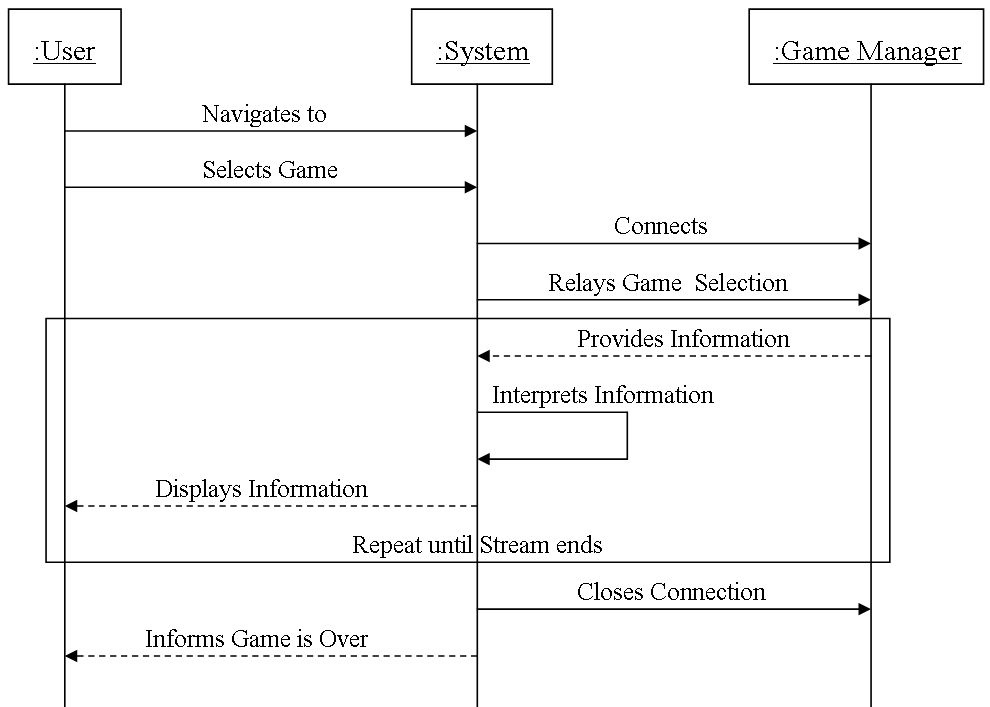
\includegraphics[width=1.0\textwidth]{./SSD_of_Watch_Live.png}
			
		\subsubsection{Description}
			Within our System Sequence Diagram, we have three actors: the User, the System, and the Game Manager. The User navigates to the game selection and selects a game to watch from the System, and the System connects to the Game Manager. The System then informs the Game Manager which game the user has selected. With a game selected, the Game Manager will provide game information to the System. The System will interpret the game information and then display this information to the User. These three steps will be repeated until the stream of game information ends. At this point, the System will close the connection with the Game Manager. Once the connection is closed, the System will notify the User that the current game is now over.
			% Incomplete
	
\newpage		% Incomplete

	%%%%%%%%%%%%%%%
% This file is concerned with the nonfunctional requirments.
%
% Please remember to compile the document from "00_finalreport.tex".
% It will not work otherwise.
%%%%%%%%%%%%%%%

\section{Nonfunctional Requirments}

	\subsection{Functionality}
	\begin{itemize}
		\item Passwords in the database repository should be encrypted to prevent breach in user privacy.
		\item All forms that write or read from the database should have some form of input validation to prevent SQL injection.
		\item User should be able to log out of users login session whenever they please.
		\item System automatically logs-out any user who has been inactive for 1 hour.
		\item All hyperlinks should transfer the user to the indicated page.
		\item The design, implementation, and support of the website, and any systems used by the website, will operate on a budget of \$0.00 per year.
	\end{itemize}
	
	\subsection{Usability}
	\begin{itemize}
		\item The website will be displayed in one of the multiple color schemes ("skins") designed for aesthetic pleasantry.
		\item Users may select a skin of their choosing, otherwise the default skin will be displayed.
		\item A single color scheme will not include colors that are difficult to distinguish for those with common forms of color blindness.
		\item All documents and code will comply with the determined style guide.
		\item Fonts should be readable from 2 feet away by an individual with average vision on a screen of 800x600 or larger resolution.
		\item Hyperlink text should appropriately represent the information to which the hyperlink leads.
	\end{itemize}
	
	\subsection{Reliability}
	\begin{itemize}
		\item User authentication will consistently log the correct user into the correct account without error.
		\item The website will never go down unless scheduled. In the case of scheduled down time, the website will display a notification at least 48 hours prior to the down time.
		\item The database repository will be backed up every two weeks.
	\end{itemize}
	
	\subsection{Performance}
	\begin{itemize}
		\item Page loading should be minimized as much as possible, so page size should be kept as small as possible. Pages will load within 1 second.
	\end{itemize}
	
	\subsection{Supportability}
	\begin{itemize}
		\item The website and the database schema will be thoroughly documented to facilitate troubleshooting by all administrators.
		\item The website will provide a means for users to contact site administrators to report site error or issue.
		\item In the case of an error, the website will provide a friendly, helpful message telling what happened, calming the user and providing a way to inform site administrators of the problem.
		\item In the case of a database error, an event will be logged for administrator use.
	\end{itemize}

\newpage		% Incomplete

	%%%%%%%%%%%%%%%
% This file is concerned with the domain analysis.
%
% Please remember to compile the document from "00_finalreport.tex".
% It will not work otherwise.
%%%%%%%%%%%%%%%

\section{Domain Analysis}

	\subsection{Diagram}
		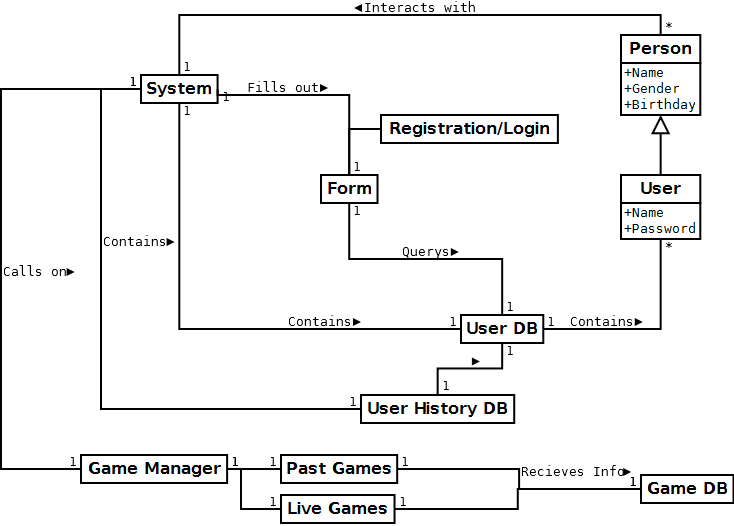
\includegraphics[width=1.0\textwidth]{./Diagram1.png}

	\subsection{Description}
		The diagram starts with the Person, a normal human being. The person interacts with the system (in the sense that the person is clicking links on the website and typing in fields). The System is in control of the general running of the domain. When a person wants to register or sign-in to the site, they are interacting with the Form, not directly to the database. The form is in control of handing the entered info(either login info or registration info) to the database. The User DB contains Users, being a class of Person. When the user requests to see a game, The Game Manager is pinged to pull up specific information, either Past Games or Live Games, recieving information from a Games database. the actual game data is presented from the databases maintained by the server group and outside the scope of this paradigm. 

\newpage			% Incomplete

	%%%%%%%%%%%%%%%
% This file is concerned with the interaction diagram.
%
% Please remember to compile the document from "00_finalreport.tex".
% It will not work otherwise.
%%%%%%%%%%%%%%%

\section{Interaction Diagrams}
	
	\subsection{Navigates to System}
	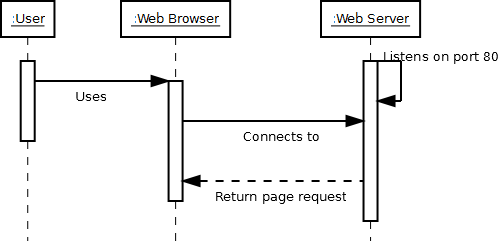
\includegraphics[width=0.50\textwidth]{./Interact1.png}
	
	This is a low coupling principle. The user uses their web browser which then interacts with our web server to display any information we intend to send.
	
	\subsection{Select Game}
	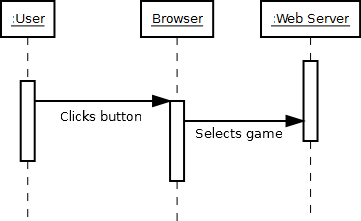
\includegraphics[width=0.50\textwidth]{./Interact2.png}
	
	Same principle as above. The user slects a game.
	
	\subsection{Connects}
	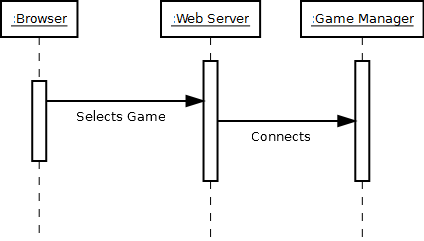
\includegraphics[width=0.50\textwidth]{./Interact3.png}
	
	High cohesion, The web server only deals with sending info to the browser, the game manager is responsible for all else.
	
	\subsection{Relays game selection}
	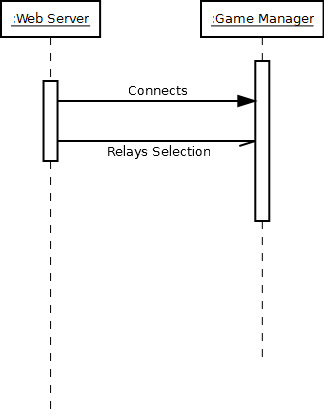
\includegraphics[width=0.50\textwidth]{./Interact4.png}
	
	This would full under the controller principle. Web server connected to the game manager and then passed alone the information that game manager needs to continue.
	
	\subsection{Provides information}
	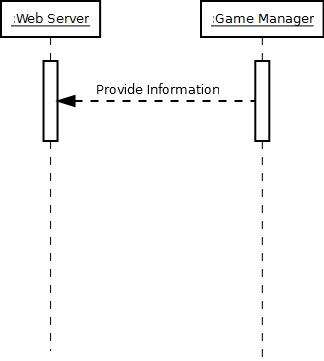
\includegraphics[width=0.50\textwidth]{./Interact5.png}
	
	Game manager provides the requested information to the web server to pass alone to user.
	
	\subsection{Interpret}
	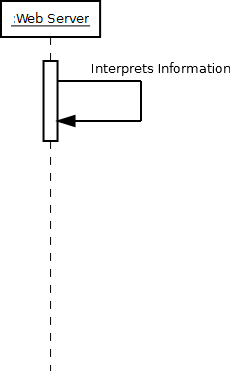
\includegraphics[width=0.50\textwidth]{./Interact6.png}
	
	It is now the web servers job to interpret the data that was passed to it.
	
	\subsection{Display}
	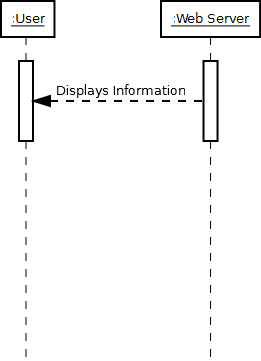
\includegraphics[width=0.50\textwidth]{./Interact7.png}
	
	Web server sends the translated information to the users browser to be displayed.
	
	\subsection{Close}
	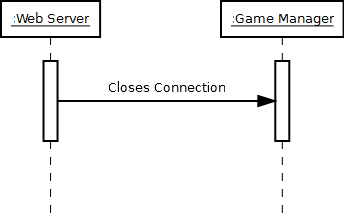
\includegraphics[width=0.50\textwidth]{./Interact8.png}
	
	The task is complete so the web server closes the connetion to the game manager.
	
	\subsection{Inform}
	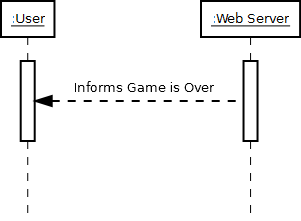
\includegraphics[width=0.50\textwidth]{./Interact9.png}
	
	Web server tells the user it has closed game session.

\newpage
	% Incomplete

	%%%%%%%%%%%%%%%
% This file is concerned with the implementation section.
% Another large section. broken up for orginization.
%
% Please remember to compile the document from "00_finalreport.tex".
% It will not work otherwise.
%%%%%%%%%%%%%%%

\section{Implementation}
	
	%%%%%%%%%%%%%%%
% This file is concerned with the style guide,
% a subsection of the implementation section.
%
% Please remember to compile the document from "00_finalreport.tex".
% It will not work otherwise.
%%%%%%%%%%%%%%%

	\subsection{Style Guide}
	
		\subsubsection{Indentation, Line length and Whitespace}
		\begin{itemize}
			\item Use tabs, not spaces, for indentation. Set tabs to equal four spaces.
			\item Braces should appear on the line below their preceding argument, indented to the same level. All code contained within the braces should be indented by one additional tab.
			\item The contents of $<$php? ?$>$ tags should always be indented. The contents of HTML and JavaScript tags may or may not be indented depending on their scope. For example, in HTML the contents of a $<$div$>$ should be indented while the contents of a $<$p$>$ should not. In JavaScript, the contents of a $<$form$>$ should be indented while the contents of an $<$option$>$ should not. The properties of a CSS selector should be indented.
			\item Line length should not exceed 85 characters. When using HTML $<$p$>$ tags to display text, the contents of the paragraph do not need to comply with line length limits. If the line exceeds 85 characters, the $<$/p$>$ tag should be placed on the line below the textual content of the paragraph.
			\item Methods containing more than 30 lines of code are discouraged. If a method is over 30 lines of code, it can probably be written more efficiently and/or broken down into multiple methods.
			\item Readability is a priority over small file sizes; use of whitespace is encouraged where appropriate.
		\end{itemize}
			
		\subsubsection{Naming Conventions}
		\begin{itemize}
			\item Filenames should not contain capital letters. Underscores are only used for pages that pass information from the client to the server. These pages should have a shared, meaningful name followed by \_form or \_post to indicate whether the page is collecting information (\_form) or processing information (\_post).
			\item CSS specifications should not contain capital letters or underscores. Use of dashes is discouraged, though it is allowed if appropriate. ID and class names should refer to the contents rather than the appearance of an element. For example, "errormsg" is preferable to "smallredtext" in the interests of maintainability.
			\item Variable names in PHP and JavaScript should use camel casing. The names of boolean variables should begin with "is."
		\end{itemize}
			
		\subsubsection{Structure of Pages}
		\begin{itemize}
			\item All displayable pages on the VirPong website will begin and end with PHP tags to include the header and footer.
			\item All textual content will be placed within HTML $<$p$>$ tags, with the exception of headers which will be within the header tag of the appropriate level (e.g. $<$h1$>$).
			\item All HTML and CSS code will comply with the W3C validators in an effort to maximize cross-browser compatibility.
		\end{itemize}
			
		\subsubsection{Documentation Conventions}
		\begin{itemize}
			\item HTML comments should be formatted like so:\\$<$!-- This is a comment. --$>$\\
			\\CSS, PHP, and Javascript comments may be formatted in either of the following two ways:\\/**\\  $*$ This is a comment. \\ $*$ Generally used at the beginning of a block of code to explain\\ $*$ its overall function in plain English.\\ $*$/\\or\\// This is a comment. \\ // Generally used within blocks of code to explain how certain\\// elements are being used. \\// Generally does not take up more than one line -- if you\\// have that much to say, consider a block comment.
		\end{itemize}
			
		\subsubsection{HTML Specific}
		\begin{itemize}
			\item All HTML tags and attributes will be entirely in lowercase.
			\item All opening HTML tags will be accompanied by a corresponding closing tag. When using multiple tags, all elements will be properly nested (e.g. $<$b$>$$<$i$>$text$<$/i$>$$<$/b$>$ rather than $<$b$>$$<$i$>$text$<$/b$>$$<$/i$>$). All singleton tags will be closed with a space and an ending slash at the end of the tag (e.g. $<$br /$>$).
			\item Attributes inside of HTML tags should be contained within double quotes. There should be no spaces between the attribute, the equals sign, and the definition. When defining multiple attributes, they should be separated by a single space.
			\item All image tags will contain an alt attribute.
			\item Div layers are generally preferable to tables and iframes. Divs will be used to display the main site layout. Tables should only be used in select cases, such as to display the contents of the database. Iframes should never be used.
		\end{itemize}
			
		\subsubsection{CSS Specific}
		\begin{itemize}
			\item All CSS will be contained in the external stylesheet rather than included as inline style.
			\item When defining styles for specific elements, think carefully about whether the selector should be an ID or a class. Elements that are only used once on each page (e.g. the content div) should use IDs; elements that may be repeated (e.g. the errormsg) should use classes.
			\item All text sizes should be specified using ems, not pixels.
		\end{itemize}
			
		\subsubsection{PHP Specific}
		\begin{itemize}
			\item Control statements (if, for, while, switch, etc.) should have one space between the control keyword and the opening parenthesis, to distinguish them from function calls.
			\item Long if statements may be split onto several lines to comply with line length limits. The conditions should be indented by one additional tab with the logical operators (e.g. \&\&) at the beginning of the line. The first condition may be indented to align with the others. The closing parenthesis and opening brace get their own line at the end of the conditions.
			\item Literal strings should be contained within singled quotes. When a literal string contains apostrophes, it should instead be contained within double quotes. SQL statements may be contained within double quotes whether or not they contain apostrophes.
			\item String concatenation will be done using the "." operator with spaces on both sides. When string concatenation exceeds line length limits, the statement should be broken up such each successive line begins with the "." operator aligned under the initial "=" operator.
		\end{itemize}
			
		\subsubsection{JavaScript Specific}
		\begin{itemize}
			\item Any JavaScript code that defines functions should be kept in an external .js file.
		\end{itemize}
			
		\subsubsection{Sources}
			\indent http://na.isobar.com/standards/ \\
			\indent http://pear.php.net/manual/en/standards.php
		% Incomplete
	
	% Does this one really belong here?
	%%%%%%%%%%%%%%%
% This file is concerned with design patterns,
% a subsection of the implementation section.
%
% Please remember to compile the document from "00_finalreport.tex".
% It will not work otherwise.
%%%%%%%%%%%%%%%

	\subsection{Design Patterns}
	
		\subsubsection{Pattern Name - Home Link}
			\begin{description}
				\item[Intent] To always provide the user with a simple path to the website's home page.
				\item[Implementation] The VirPong logo in the upper left corner of the layout is a hyperlink to the VirPong home page. This is present on every page.
				\item[Consequences] Allows users to navigate to the home page no matter what page they start at. This is especially helpful if users arrive at the website via a search engine or an emailed link to a specific page.
				\item[Related Patterns] Main Navigation, Footer Bar
				\item[Pattern Name] Main Navigation
				\item[Intent] To always provide the user with hyperlinks to all areas of the website.
				\item[Implementation] The horizontal bar at the top of the layout is a menu containing dropdowns with links to different pages of the VirPong website. This is present on every page.
				\item[Consequences] Allows users to navigate to a page of their choosing no matter what page they start at.
				\item[Related Patterns] Home Link, Footer Bar
			\end{description}
			
		\subsubsection{Pattern Name - Footer Bar}
			\begin{description}
				\item[Intent] To always provide the user with hyperlinks to important informational content regarding the use of the system.
				\item[Implementation] The centered bar at the bottom of the layout is a footer containing links to important information regarding the services that VirPong provides. These links are: about us, contact us, privacy policy, terms of use, and code of conduct. This is present on every page.
				\item[Consequences] Allows users to directly access information about the service no matter what page they start at.
				\item[Related Patterns] Home Link, Main Navigation
			\end{description}
			
		\subsubsection{Pattern Name - Account Registration}
			\begin{description}
				\item[Intent] To only display protected content to users who have registered with the service. To store user information which can later be used to enhance the user experience.
				\item[Implementation] Users must fill out the registration form before they can play VirPong games, participate in tournaments, or use the chat feature.
				\item[Consequences] Allows for personalization of the VirPong experience, including display of personal player history information, the ability to chat with other users, email notifications regarding tournament participation, and happy birthday emails. Trade-offs include potential loss of users who are discouraged by the registration form.
				\item[Related Patterns] Lazy Registration, Log In, Input Feedback
			\end{description}
			
		\subsubsection{Pattern Name - Lazy Registration}
			\begin{description}
				\item[Intent] To allow users to become familiar with the service before requiring them to register.
				\item[Implementation] Users can watch VirPong matches (both live and past matches) and view high score information without being registered or signed in to an account. Users can also access all informational content (about us, contact us, privacy policy, terms of use, code of conduct, rules, system requirements, news) without being registered or signed in to an account.
				\item[Consequences] Allows users to try out the system with little immediate commitment, making registration seem like more of a choice than a chore. Allows users to be already invested in VirPong by the time they register for an account, making it more likely that our registered users are active uses. Trade-offs include potential loss of registered accounts by users who only utilize features that do no require registration.
				\item[Related Patterns] Account Registration
			\end{description}
			
		\subsubsection{Pattern Name - Log In}
			\begin{description}
				\item[Intent] To identify a registered user in order to properly personalize their experience.
				\item[Implementation] The main navigation contains a link to the log in form, allowing registered users to authenticate into the system whenever they desire. If an unauthenticated user attempts to access a page that is only available to registered users, it will display a prompt asking the user to log in before proceeding.
				\item[Consequences] Allows for personalization of the VirPong experience, including unlocking access to certain pages that are only available to registered users.
				\item[Related Patterns] Account Registration
			\end{description}
			
		\subsubsection{Pattern Name - Input Feedback}
			\begin{description}
				\item[Intent] To communicate with users about information they are submitting to the service.
				\item[Implementation] All improperly filled out forms will generate specific error messages, whether through Javascript alerts or inline text. All properly filled out forms will lead to a success message, confirming that the user?s submission was successful. This design pattern applies to the registration, log in, and account settings forms.
				\item[Consequences] Prevents improper information submission by alerting the user immediately and directly of any errors. Allows the user to feel confident upon receipt of success message that their information has been passed to the system.
				\item[Related Patterns] Account Registration, Good Defaults
			\end{description}
			
		\subsubsection{Pattern Name - Good Defaults}
			\begin{description}
				\item[Intent] To prevent users from having to type any more keystrokes than strictly necessary by prefilling certain form values to anticipate the user input.
				\item[Implementation] The account settings form automatically fills in the user?s current first name, last name, email address, birthday, and gender. The user can then edit any fields he wants to change and leave any fields he wants to remain the same.
				\item[Consequences] Eliminates the need for the user to reenter all of their information in order to change any field, resulting in significantly increased convenience for the user. Trade-offs include reminding users that we have their personal information and we know how to use it.
				\item[Related Patterns] Input Feedback
			\end{description}
	% Incomplete
	
	%%%%%%%%%%%%%%%
% This file is concerned with the implementation section.
%
% Please remember to compile the document from "00_finalreport.tex".
% It will not work otherwise.
%%%%%%%%%%%%%%%

	\subsection{Installation}
		There are a few requirements to installing and using our application. Our development platform is Ubuntu and the following are requirements for the installation:
		\begin{description}
			\item[Install a LAMP Server] A LAMP server is composed of a Linux environment, and installations of Apache, MySQL and PHP. However, this step is outside the scope of our tutorial, but you may follow this guide:\\http://www.howtoforge.com/ubuntu\_debian\_lamp\_server
			\item[Install git] Both our application and Node.js are hosted on git, so it is important to install git on your machine. Installation of git will be covered in the next requirement
			\item[Install Node.js] This is how we are going to run our Javascript on the server. You can follow these directions here to install Node.js:\\http://howtonode.org/how-to-install-nodejs
			\item[Install NPM] NPM is a package manager and has become the standard for installing node libraries. We are going to use this to install socket.io, and you can install NPM by entering the following command in your terminal window 'curl http://npmjs.org/install.sh | sh'
			\item[Install Socket.io] This is how we are going to create bidirectional communication between the server and browser. To install, enter the following command in your terminal window: 'npm install socket.io'
		\end{description}
		Prior to installing the VirPong web application, the database needs to be configured to match the database used with the VirPong game. Once the MySQL database is installed, do the following:
		\begin{enumerate}
			\item Log into your MySQL database. From your terminal window:
			\begin{enumerate}
				\item enter 'mysql -u $<$your\_username$>$ -p'
				\item press enter
				\item enter '$<$your\_password$>$'
				\item press enter
			\end{enumerate}
			\item Now that you're logged into MySQL, the database needs to be created. From the MySQL prompt, enter the following command:\\'CREATE DATABASE db2'
			\item This creates the database, but tables must be created within the database. To create the three tables that are used in the VirPong game, enter the following three commands into the MySQL prompt
			\begin{enumerate}
				\item create table GamesPlayed (gameID INT(10) NOT NULL AUTO\_INCREMENT, username1 VARCHAR(50) NOT NULL, username2 VARCHAR(50) NOT NULL, score1 TINYINT NOT NULL, score2 TINYINT NOT NULL, win TINYINT NOT NULL, INDEX index1(gameID), CONSTRAINT FK\_customer FOREIGN KEY(username1) REFERENCES customer(username), CONSTRAINT FK\_customer\_2 FOREIGN KEY(username2) REFERENCES customer(username));
				\item create table Customer (username VARCHAR(50) NOT NULL, password VARCHAR(50) NOT NULL, firstname VARCHAR(50) NOT NULL, lastname VARCHAR(50) NOT NULL, email VARCHAR(256) NOT NULL, birthday DATE NULL, gender TINYINT NULL, PRIMARY KEY(username));
				\item create table Registration (gameID INT NOT NULL AUTO\_INCREMENT, username1 VARCHAR(50) NOT NULL, username2 VARCHAR(50) NOT NULL, gameTime DATETIME NOT NULL, tournamentID INT NULL,  INDEX index1(gameID), CONSTRAINT FK\_customer FOREIGN KEY(username1) REFERENCES customer(username), CONSTRAINT FK\_customer\_2 FOREIGN KEY(username2) REFERENCES customer(username));
			\end{enumerate}
			\item With all three tables created, exit the MySQL prompt to continue the installation process, by entering:\\'exit'
		\end{enumerate}
		With all of the requirements installed as well as the MySQL database, we can begin running the application. To get the source code for our application:
		\begin{enumerate}
			\item Navigate in your terminal window to your Apache root folder (by default, this is /var/www):\\'cd /./var/www'
			\item Clone our source code by issuing the following command in your terminal window:\\'git clone git://github.com/VirPong/human-pong.git'
			\item Navigate to into the Communication folder:\\'cd human-pong/WebUI/site/http/communication'
			\item Run the VirPong web server by issuing command in your terminal window:\\'node server.js'\\Note: The client.js code may need to be changed depending on your system configuration. Simply change open the client.js file and change the IP address to the address of your server. ex: 'socket = io.connect('xxx.xxx.xxx.xxx');' With your server's address in the parenthesis
			\item To view the application in use, point your web browser to: 'http://localhost/human-pong/WebUI/site/http/communication/index.html'
		\end{enumerate}
		To incorporate this HTML file into your own application, simply follow the steps above and create a link from your website to the Live Game page by making a link in your HTML file to the index.html file.\\To find further instructions on how to install the VirPong platform, or to find other resources that pertain to VirPong, please visit our repository and wiki page at: https://github.com/VirPong/human-pong
		% Incomplete
	
	\subsection{ER Diagram}
		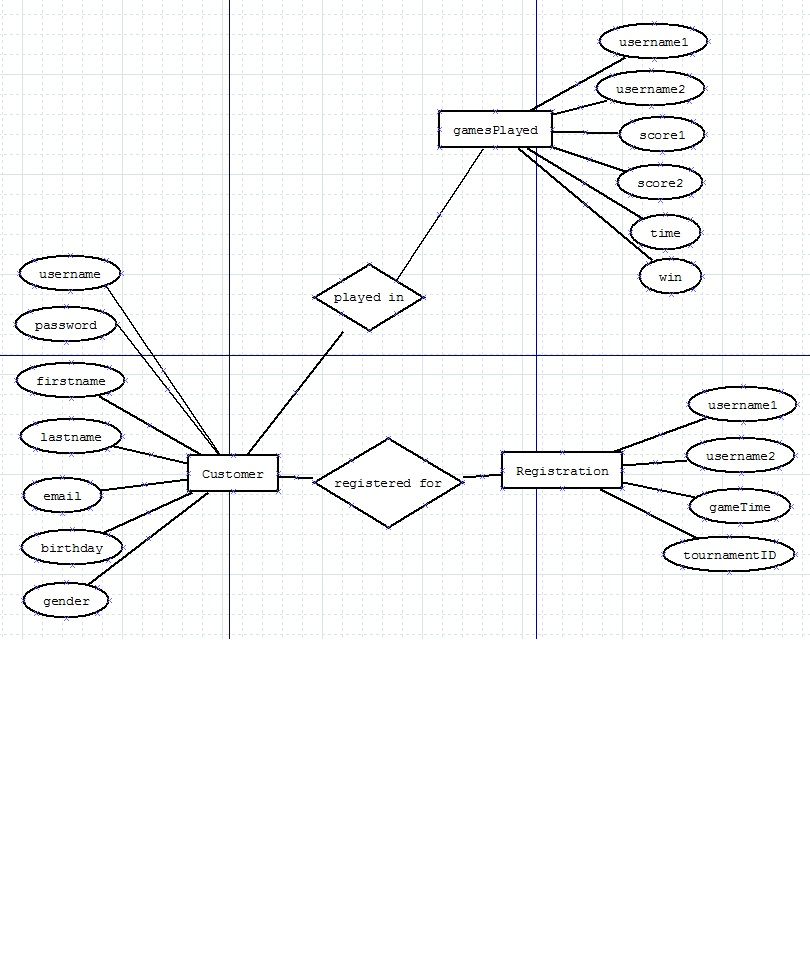
\includegraphics[width=1.0\textwidth]{./ER.jpg}
	
	%%%%%%%%%%%%%%%
% This file is concerned with the data storage,
% a subsection of the implementation section.
%
% Please remember to compile the document from "00_finalreport.tex".
% It will not work otherwise.
%%%%%%%%%%%%%%%

	\subsection{Data Storage}
		Within the website's database, we have established three different classes of information that we will be storing: information provided by the client that is related to the world outside of VirPong, information specified by the client that will identify the client within the VirPong world, and information recorded about game play or game statistics. Among the information in the personal class, is their full name, their email address, their birthday, and their gender. Our website's database second class stores information that is unique to our clients and is just as sensitive as their personal information. Among this class of information is our client?s username, their password, the games that they have played, and the times that they have played these games at. The rest of the data that we store in the website's database makes up a third class of information, information that pertains to VirPong games. The data associated with this class includes unique game ID's, the game times, and scores of games, and who won a specific game. Although we have three specific classes of data that we are storing, some of the data exists in multiple classes, such as the times that users have played games, and their specified username and passwords.


		\subsubsection{Database Schema:}
			\begin{description}
				\item[Table:] Customer twice

				\begin{center}
					\begin{tabular}{ | l | l | l | l | l | l|}
						\hline
						Field & Type & Null & Key & Default & Extra \\ \hline \hline
						username & varchar(50) & NO & PRI & NULL & \hspace{1 pc} \\ \hline
						password & varchar(50) & NO & \hspace{1 pc} & NULL &\hspace{1 pc}  \\ \hline
						firstname & varchar(50) & NO & \hspace{1 pc}& NULL &\hspace{1 pc}  \\ \hline
						lastname & varchar(50) & NO &\hspace{1 pc} & NULL &\hspace{1 pc}  \\ \hline
						email & varchar(256) & NO &\hspace{1 pc} & NULL &\hspace{1 pc}   \\\hline
						birthday & date & YES &\hspace{1 pc} & NULL & \hspace{1 pc} \\ \hline
						gender & tinyint(4) & YES &\hspace{1 pc} & NULL &\hspace{1 pc}  \\
						\hline
					\end{tabular}
				\end{center}

				\item[username:] This is the primary key for the Customer database and therefore cannot be null. This will store the user names specified by our customers.
				\item[password:] This field stores the password for the customer. This field cannot be null because it is important for us to maintain the ability to authenticate all users.
				\item[firstname:] This field stores the user?s first name. This field cannot be null because we would like to identify our users by sending them personal messages.
				\item[lastname:] This field stores the user?s last name. This field also cannot be null because we would like to also include the last name of our customer in our personal messages.
				\item[email:] This field stores the email address for the user. We will be sending notifications of future games and must have the ability to contact our customers, therefore this field cannot be null.
				\item[birthday:] This field will store the birthday of our customer. This field can be null if the user would like.
				\item[gender:] This field stores the gender of the customer. This field can be null if the user would like.
			\end{description}

			\begin{description}
				\item[Table:] GamesPlayed

				\begin{center}
					\begin{tabular}{ | l | l | l | l | l | l|}
						\hline
						Field & Type & Null & Key & Default & Extra \\ \hline \hline
						gameID & int(10) & NO & MUL & NULL & auto\_increment \\ \hline
						username1 & varchar(50) & NO & MUL & NULL &\hspace{1 pc}  \\ \hline
						username2 & varchar(50) & NO & MUL& NULL &\hspace{1 pc}  \\ \hline
						score1 & tinyint(4) & NO &\hspace{1 pc} & NULL &\hspace{1 pc}  \\ \hline
						score2 & tinyint(4) & NO &\hspace{1 pc} & NULL &\hspace{1 pc}   \\\hline
						win & tinyint(4) & NO &\hspace{1 pc} & NULL & \hspace{1 pc} \\
						\hline
					\end{tabular}
				\end{center}
				
				\item[gameID:] This is the key for the GamesPlayed table and it allows us to uniquely identify each game played. This field is automatically incremented by the database.
				\item[username1:] This stores the user name of one of the customers that played in this match. This will never be null since we know the users that played in the game.
				\item[username2:] This stores the user name of one of the customers that played in this match. This will never be null since we know the users that played in the game.
				\item[score1:] This will store username1?s final score. This field will not be null since we need to know the player?s scores.
				\item[score2:] This will store username2?s final score. This field will not be null since we need to know the player?s scores.
				\item[win:] This field will denote the winner, with either a 1 or a 2 depending on the number of the user that won, of the game played.

			\end{description}
				
			\begin{description}
				\item[Table:] Registration
				
				\begin{center}
					\begin{tabular}{ | l | l | l | l | l | l|}
						\hline
						Field & Type & Null & Key & Default & Extra \\ \hline \hline
						gameID & int(11) & NO & MUL & NULL & auto\_increment \\ \hline
						username1 & varchar(50) & NO & MUL & NULL &\hspace{1 pc}  \\ \hline
						username2 & varchar(50) & NO & MUL& NULL &\hspace{1 pc}  \\ \hline
						gameTime & datetime & NO &\hspace{1 pc} & NULL &\hspace{1 pc}  \\ \hline
						tournamentID & int(11) & YES &\hspace{1 pc} & NULL &\hspace{1 pc}   \\
						\hline
					\end{tabular}
				\end{center}

				\item[gameID:] This is the key for the Registration table and it allows us to uniquely identify each upcoming game. This field is automatically incremented by the database.
				\item[username1:] This stores the user name of one of the customers playing in this match. This will never be null since these are established future game with two users.
				\item[username2:] This stores the user name of one of the customers playing in this match. This will never be null since these are established future game with two users.
				\item[gameTime:] This field stores the date and time for the future match to occur.
				\item[tournamentID:] This field is used to denote whether a game is part of a tournament. By allowing a null value for tournamentID, we are able to show that a game isn?t a tournament game, and when the game is a tournament game, we can specify that it is a tournament game, as well as  which tournament game, by inserting that tournament?s numeric ID.
			\end{description}

			\textbf{Reasoning for this design choice:}
				We chose to design our database this way so that we have tables that are specific to the role that the tables are playing. We chose this path because we did not want to have all of our data stored in a single table, which would cause inconsistencies in inserting data into the table. The Customer table is created with information that is specific to identifying our client, as well as personal information that will benefit their VirPong experience. The GamesPlayed table contains information about games that have already been played, including the final score of the game, and who won the game. The Registration table contains data about upcoming games.\\
				In our Customer table, we have elected to store a client?s identifying information such as their first name, last name, and user name. We also store a password, because we want to maintain that people that are logged into our site are registered users. We also store information such as email addresses, to notify our clients of upcoming events or registered games, as well as client birthdays to wish clients happy birthdays. The email field is also 256 characters long, because this is the longest possible length of an email address.\\
				The Games Played table holds information specific to games that have been played in the past. Within the table, we store the ID of the game that has been played, so we can uniquely identify games. We also store the names of both users so we can display the players in a certain game, as well as the win field, which references the winning player, so we can determine game statistics. The table also stores the score for each player so we can follow the scores of certain players, as well as the scores for an individual game.\\
				The last table, Registration holds data that is used to plan a game in advance. We use a game ID to uniquely identify the games in question, but also require the use of a Game Time so that we can remind players when a game is upcoming, as well as to have absolute times for when games are to occur. We also store the names of both players, which we can use to reference the Customer table, to send notifications to the players, as well as advertise which players are about to play a game. The last field, the tournament ID is also used to tell whether or not a certain game is part of a tournament. The field allows an input of null, so when a certain game is not part of a tournament, we can specify null.
			% Incomplete
	
	%%%%%%%%%%%%%%%
% This file is concerned with testing and verification,
% a subsection of the implementation section.
%
% Please remember to compile the document from "00_finalreport.tex".
% It will not work otherwise.
%%%%%%%%%%%%%%%

	\subsection{Testing and Verification}
	
		The testing and verification for the VirPong website will be through validators and various kinds of testing. All the HTML and CSS code will be ran through the W3C validators available online. They will check for the indicated doctype syntax compliance of all of our scripts and compare them against the XHTML 1.1 standard. For all other types of scripts we will be using Google�s developer tools in Google Chrome to see resource load times and any errors thrown by the scripts.\\
		
		We plan on performing four types of testing upon our code: unit, integration, system, and regression. For the unit testing we are going to use a program called QUnit. We will then uses integration testing across multiple departments of code. Then we will do some system testing against all of our requirements. In this stage of testing we will test scripts in the latest versions of Microsoft�s Internet Explorer, Mozilla�s Firefox, Apple�s Safari, and Google�s Chrome on a Windows 7 machine and a Ubuntu distribution of Linux. We will also report on each functionalities success on each platform and browser to report to the user. Lastly we will perform regression testing when we make additional releases of the software to make sure they implement all functions.
			% Incomplete

\newpage		% Incomplete

	%%%%%%%%%%%%%%%
% This file is concerned with the reflections section.
%
% Please remember to compile the document from "00_finalreport.tex".
% It will not work otherwise.
%%%%%%%%%%%%%%%

\section{Reflections}

	\subsection{Challenges}
	
		\subsubsection{Server/Client Communication}
			One of the main challenges that we faced in creating a method of viewing VirPong games was in the actual communication between the server and the client. In the past, there have only been a handful of ways that developers have tackled the issues of browser communication including the use of making a �connection� via a port opening by Flash, or through Reverse AJAX. However, both of these techniques had disadvantages that we wanted to avoid, so we elected to use a newer technology, WebSockets, specifically the Socket.io framework for Javascript. The challenge that came along with this route is the newness of Socket.io as well as Node.js, which we use in conjunction of Socket.io. Looking for online tutorials, we found many tutorials that used both of these technologies in different situations, as well as samples of code that used the two technologies in conjunction with other frameworks, making it difficult to get an understanding of how Node.js and Socket.io worked independently of these other frameworks. To overcome the issue of adopting these two new technologies, our team focused on trying to re-implement tutorial code as we found it, and upon finding working tutorial code, we would manipulate the code in attempts to break the code down into more simplistic forms. Going through this process, our team was able to achieve very simple recreations of tutorial code that we had found, providing us with an understanding of what is required in using Node.js and Socket.io.\\While this technique worked for our team, and we were able to break tutorial code down into simplified forms, and from these simplified forms determine the best way to structure our own code, we believe that we may have saved some time by investigating our options further. During this process, we explored many different methods of communication between the client and the server, however, we were eager to begin coding and would often try to implement a piece of code before pursuing alternatives. We believe that if we had pursued other examples or pieces of tutorial code, we could have shortened the amount of time, and potentially frustration, that we used to develop a working implementation of server to client communication.


		\subsubsection{Large Workload}
			One challenge that we anticipated in the Initial Plan was the sheer number of tasks that lay before us in creating a functional, attractive web user interface for VirPong. Identifying this issue early on was a key to the way we have handled the workload. By always keeping in mind the magnitude of our task, we stay motivated to produce results each and every week.\\In hindsight, this challenge may have been easier to deal with if we had planned our initial schedule more carefully. One of our proposed strategies for tackling the workload was to stick tightly to our schedule, but this proved unrealistic. Often our features relied on the existence of features from other departments -- for example, we cannot code and test pages that read information from the database of past games until we have discussed with the server department who is responsible for writing this information to the database and what the schema of the database will be. Had we been more aware of the realities of this situation, we would have placed all such features that rely on other departments further down the schedule, and we would have communicated our needs to other departments before the submission of the initial plan so that they might consider them when designing their own schedules.\\Because our schedule was at times unhelpful, rather than following it to the letter we have taken care to be proactive about getting things done. In particular, Kyle and Katie often found that the tasks assigned to them were unfeasible at the present time. Rather than shrugging it off and making no progress for the entire week, their response was to seek out alternate tasks that could be completed. In this way, we implemented Javascript validation of forms and a complete site layout more quickly than anticipated in the original schedule.\\Our other main strategy in conquering our heavy workload was splitting our team into pairs that worked together on shared tasks. In general, Aryn and Garrett have been configuring the database and working toward communication with the server while Katie and Kyle have been writing pages that access the database and focusing on the aesthetics and organization of the website. We have been happy with the buddy system, as it simultaneously holds us accountable for working on our assigned tasks and gives us another bright mind to bounce ideas off of. Working in pairs has also been quite practical, as it allows our team to tackle two problems at once. Since many of our meetings are with only the pair as opposed to the whole group, they are easier to schedule into our busy lives.

\newpage		% Incomplete

	%%%%%%%%%%%%%%%
% This file is concerned with the references section.
%
% Please remember to compile the document from "00_finalreport.tex".
% It will not work otherwise.
%%%%%%%%%%%%%%%

\section{References}

	\begin{description}
	
		\item[CSS - http://w3schools.com/css] \hfill \\
			Cascading Style Sheets is a style sheet language that can be applied to HTML. We will be using CSS to create a consistent, appealing layout across all our pages.
		\item[Github - http://github.com] \hfill \\
			Github is a hosting system for the version control system Git. We will be using Github to collaborate with each other and with the other Vir-Pong development teams.
		\item[GDocs - http://docs.google.com] \hfill \\
			Google Docs is a web-based, collaborative document editing service. We will be using GDocs to share information between team members.
		\item[HTML - http://w3schools.com/html] \hfill \\
			HyperText Markup Language is the standard markup language for web pages. We will be using HTML in conjunction with CSS and PHP to create the layout of our website.
		\item[HTML5 - http://w3schools.com/html5] \hfill \\
			HyperText Markup Language 5 is a revision of the HTML standard that includes new multimedia content. We will be using HTML5 in conjunction with JavaScript to display games of Vir-Pong on the web.
		\item[HTTP/HTTPS] \hfill \\
			Hyper Text Transfer Protocol/Hyper Text Transfer Protocol Secure is the  protocol for sending web-pages or other information across a network. HTTPS is the SSL encrypted version, providing secure communication between the web user and the server when sensitive data is being handled.
		\item[JavaScript - http://w3schools.com/js] \hfill \\
			JavaScript is a dynamic, client-side scripting language. We will be using JavaScript in our forms, including validating those forms to enhance Vir-Pong's security. We will also use JavaScript in conjunction with the Canvas element in HTML5 to produce our game display.
		\item[JWebSockets - http://jwebsocket.org/] \hfill \\
			JWebSockets is both a Java and a JavaScript implementation of HTML5's WebSockets. The use of WebSockets allows for full-duplex communications between a server and a set of clients, including websites, as well as mobile devices. We will be using JWebSockets to push information from the server to the website clients, which will include features such as live streaming of Vir-Pong games, as well as the potential for a client chat system.
		\item[\LaTeX - http://latex-project.org] \hfill \\
			\LaTeX is a document markup language for \TeX typesetting. We will be using \LaTeX to format our printed documents, such as weekly manager reports and this initial plan.
		\item[MySQL -  http://dev.mysql.com/downloads/mysql/] \hfill \\
			MySQL is  type of SQL database that stores relational information well. We are using a MySQL database to store all of our information we collect from the user, game information, and future game times.
		\item[Photoshop - http://photoshop.com] \hfill \\
			Adobe Photoshop is a graphics editing program. We will be using Photoshop to produce mockups of our site layout. We will also use Photoshop to render the Vir-Pong logo and any other graphics used on our website.
		\item[PHP - http://php.net] \hfill \\
			PHP: Hypertext Processor is a server-side scripting language that integrates smoothly with HTML. We will be using PHP on all of our web pages. We will use PHP to insert the header and footer of our layout on each page. We will also use PHP to make database queries, such as when registering a new member with our system or retrieving user information (e.g. high scores, account settings).
		\item[PHP Designer - http://mpsoftware.dk/phpdesigner.php] \hfill \\
			PHP Designer is a text editor designed specifically for writing PHP, HTML, CSS, and JavaScript. It contains useful tools for testing and debugging code in all four of these languages. We will be using PHP Designer to write much of our code for this project.
		\item[Powerpoint - http://office.microsoft.com/en-us/powerpoint] \hfill \\
			Microsoft Powerpoint is a commercial presentation program that is part of the Microsoft Office suite. We will be using Powerpoint for our weekly manager presentations in order to provide the rest of the company with a visual representation of our progress.
		\item[Various browsers] \hfill \\
		Internet Explorer: http://microsoft.com/ie \\ Mozilla Firefox: http://mozilla.org/firefox\\Google Chrome: http://google.com/chrome\\Safari: http://apple.com/safari.\\
			Web browsers allow users to navigate the World Wide Web. We will be using browsers to test our website for display and usability. For this reason, it is important that we test in all of the most popular browsers currently in use. This enables us to be sure that our site displays properly to all users, thereby keeping our client base as wide as possible.
			
	\end{description}
		% Incomplete

\end{document}
